\section{Datasets}
\label{sec:datasets}

In the course of this project, we used 3 different datasets:

\subsection{SurgToolLoc}
\label{ssec:datasets_surgtoolloc}
The dataset of the \emph{SurgToolLoc} Challenge is provided by the \emph{International Society for Computer Aided Surgery} (ISCAS). Its a result of surgical training exercises using the \emph{da Vinci} robotic system and contains \num{24695} video clips, each 30 seconds long, captured at a resolution of 1280$\times$720 pixels and 60fps, resulting in 1800 frames per video and almost 45 Million frames in total. Each video contains 3 out of 14 different tools (\ref{fig:surgtoolloc_tools}), of which not always every tool is active and visible, resulting in a certain amount of label errors. While this training dataset is only annotated with video-level tool labels, there exists a non-public test dataset additionally annotated with bounding boxes around the robotic tools. Sadly, we could not get access to this test dataset, which is why we will only test the tool classification on it and not the localization.

\begin{figure}[h]
	\centering
	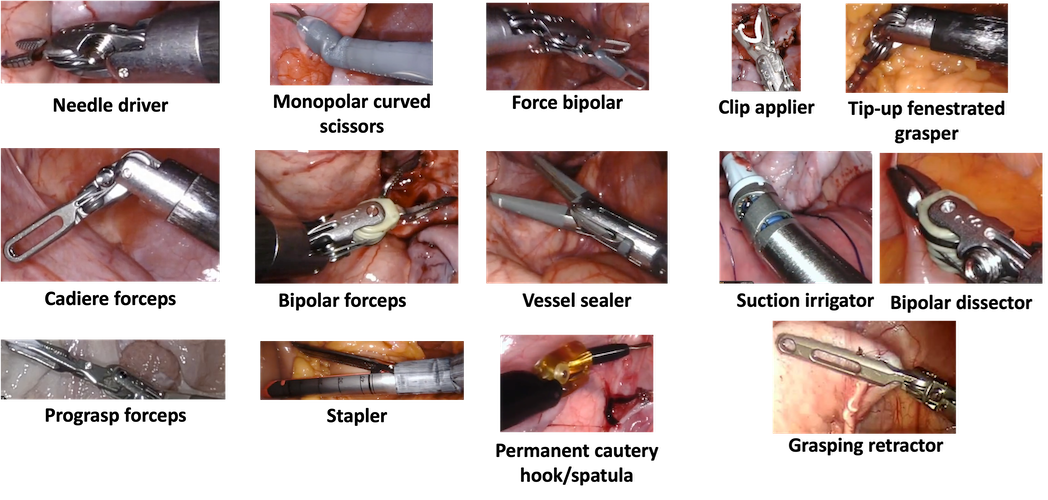
\includegraphics[width=15cm]{4_experiments/images/datasets/surgtoolloc_tools.png}
	\caption{All 14 tool classes of the \emph{SurgToolLoc} dataset.}
	\label{fig:surgtoolloc_tools}
\end{figure}

As training on such a massive dataset would have been unfeasible for our project, we created subset containing \num{10000} frames, randomly sampled from all videos and downscaled to 900$\times$620 pixels. \num{7000} of those frames were used for training and \num{3000} for testing. This re-sampling had the additional advantage of improving the extreme class-imbalance in the original data, where the most frequent class occurred \num{1000} times more often the least one (\ref{fig:surgtoolloc_tool_frequencies}).

\begin{figure}[h]
	\centering
	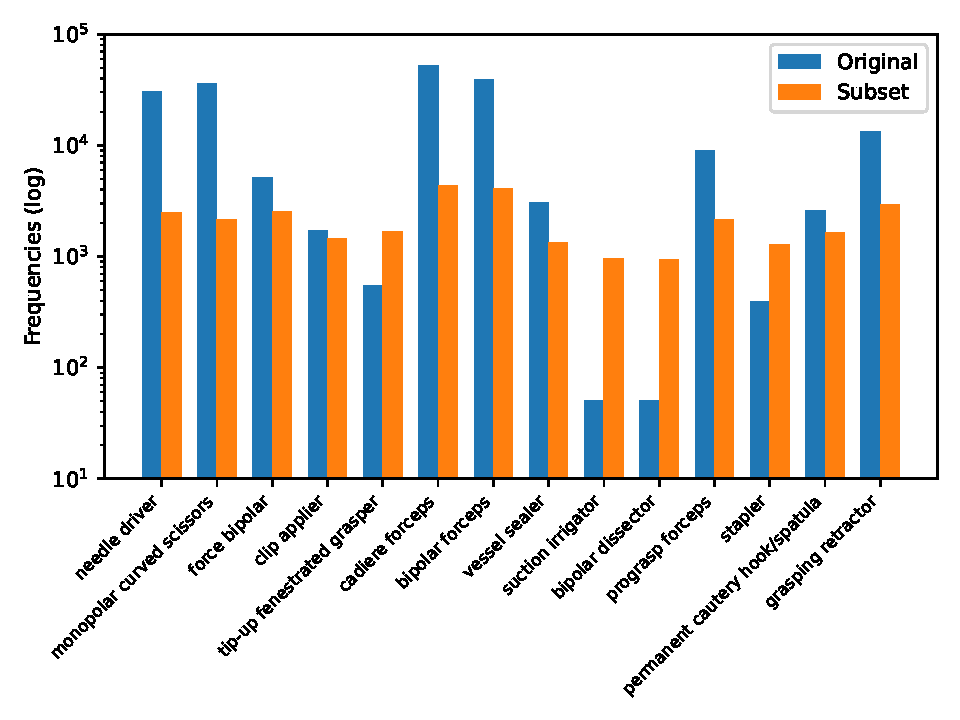
\includegraphics[width=15cm]{4_experiments/images/datasets/surgtoolloc_frequencies.pdf}
	\caption{Tool frequencies of the \emph{SurgToolLoc} dataset (video-level) and its subset (frame-level).}
	\label{fig:surgtoolloc_tool_frequencies}
\end{figure}

\subsection{Cholec80}
The \emph{Cholec80} dataset \cite{endonet} is provided by the \emph{CAMMA} research group at the University of Strasbourg and contains 80 videos of cholecystectomy surgeries, which combined result in about \num{180000} frames, most of them captured at resolution of 854$\times$480 pixels. It includes 7 different tool classes (\ref{fig:cholec80_tools}), from which a frame contains 0 to 3 and on average $1.32$ instances. In contrast to the \emph{SurgToolLoc} dataset, \emph{Cholec80} is annotated with frame-level tool labels, resulting in much less label errors. Bounding box labels were generated for the publication \cite{Vardazaryan}, but to our knowledge, have not been published.

\begin{figure}[h]
	\centering
	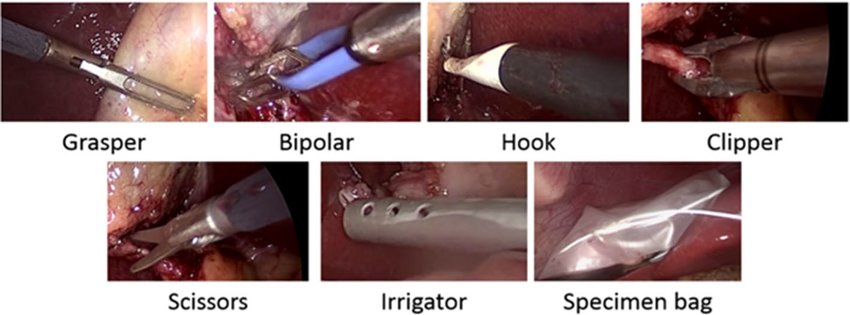
\includegraphics[width=13cm]{4_experiments/images/datasets/cholec80_tools.jpg}
	\caption{All 7 tool classes of the \emph{Cholec80} dataset.}
	\label{fig:cholec80_tools}
\end{figure}

Similar to before, this number of frames would have been unmanageable for us, so we again created a subset, of this time 6000 frames, randomly sampled from all classes. While in the original set, the factor between the least and most appearing tool is about 30, it's only 4.5 in the subset. A complete class-balance would be hard to achieve, as some of the tools, like the Grasper, almost exclusively are used with the other tools together.


\subsection{M2CAI16}

The \emph{M2CAI16} dataset contains \num{2811} frames (\num{2248} for training and \num{563} for testing) gathered from the videos 61-76 in \emph{Cholec80}. Every frame is fully annotated with tool presence labels and bounding boxes. Its size makes it manageable for us and its bounding box annotations can be used to evaluate the tool localization, which is why we will mainly use it for the following experiments.


\begin{figure}[h]
	\makebox[\linewidth][c]{
		\begin{subfigure}[b]{.6\textwidth}
			\centering
			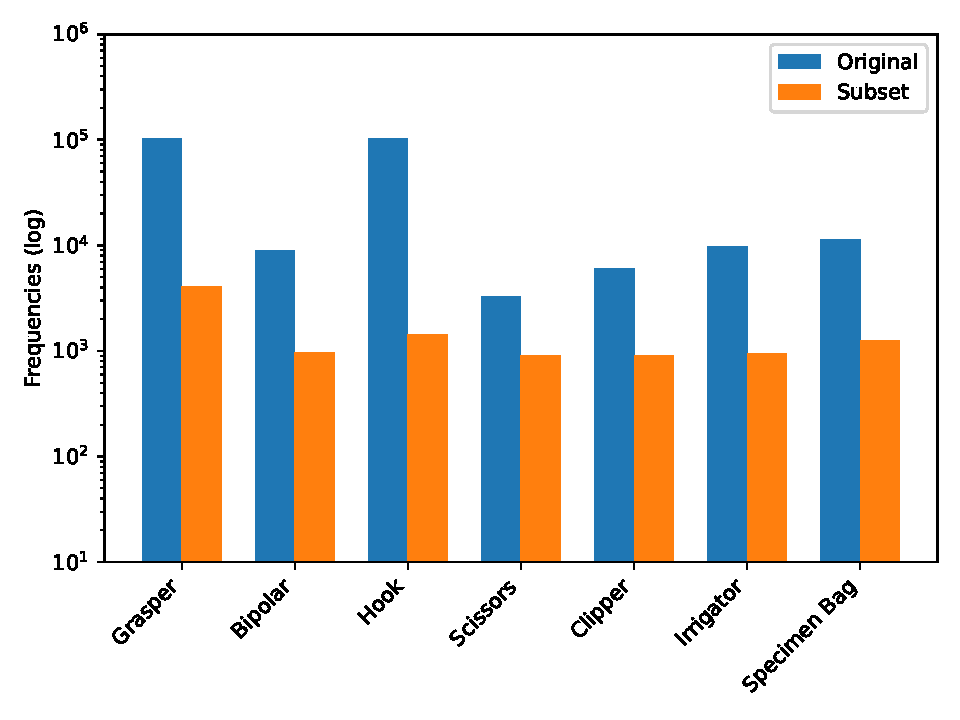
\includegraphics[width=9cm]{4_experiments/images/datasets/cholec_frequencies.pdf}
			\label{fig:cholec80_frequncies}
		\end{subfigure}%
		\begin{subfigure}[b]{.6\textwidth}
			\centering
			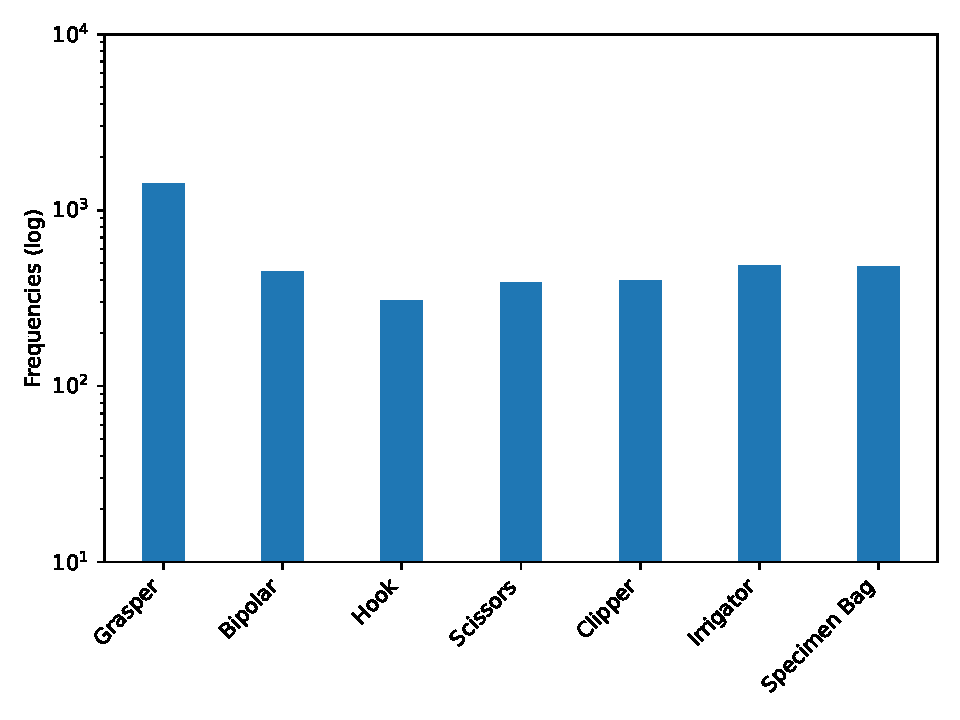
\includegraphics[width=9cm]{4_experiments/images/datasets/m2cai16_frequencies.pdf}
			\label{fig:m2cai16_frequencies}
		\end{subfigure}
	}
	\caption{(left) Frame-level tool frequencies of the \emph{Cholec80} dataset and its subset \\(right) Frame-level tool frequencies of the \emph{M2CAI16} dataset}
\end{figure}


\section{Experimental Setups}

In the following, we will define a set of standard parameters that can the be used as baseline to compare different parameter setups. All of them will have in common, that the model will be a fully convolutional neural network consisting of a backbone, an additional convolutional layer with (1$\times$1) kernel and a spatial pooling in the end. The stride of the last two convolutional layers of the backbone will vary. As optimizer we will use Stochastic Gradient Descent with momentum and weight decay. The learning rate will be reduced stepwise by a factor $\gamma$ and can be specified independently between the backbone (lr$_1$) and convolutional layer (lr$_2$). The train loss is calculated with class weights according to this formula
\[w_c = \frac{m}{F_c}\]
where $w_c$ is the corresponding weight of class $c$, $m$ is the median frequency across all tools and $F_c$ the frequency of $c$ \citep{lstm}.

\subsection{Standard Parameters}

\cite{Vardazaryan} and \cite{lstm} both worked with the following hyperparameters:

\begin{center}
	\begin{tabular}{ c | c }
		lr$_1$, lr$_2$ & 0.001, 0.1\\  
		$\gamma$ & 0.1\\
		weight decay & $10^{-4}$\\
		\color{gray}momentum & \color{gray}0.9\\
		\color{gray}strides & \color{gray}1, 1\\
		\color{gray}backbone & \color{gray}ResNet18\\
		\color{gray}pooling & \color{gray}WildCat
	\end{tabular}
\end{center}

They chose to train the backbone with a learning rate 100 times smaller than the one of conv. layer to account for its pretraining on the ImageNet dataset.\\

However, by tuning lr$_1$, lr$_2$, $\gamma$ and weight decay using Gaussian Processes, we came up with the following set:

\begin{center}
	\begin{tabular}{ c | c }
		lr$_1$, lr$_2$ & 0.01, 0.01\\  
		$\gamma$ & 0.45\\
		weight decay & $10^{-3}$\\
		\color{gray}momentum & \color{gray}0.9\\
		\color{gray}strides & \color{gray}1, 1\\
		\color{gray}backbone & \color{gray}ResNet18\\
		\color{gray}pooling & \color{gray}WildCat
	\end{tabular}
\end{center}

As can be seen, lr$_1$ should start 10 times higher and lr$_2$ 10 times lower, so that they start at the same value, with the reduction factor $\gamma$ being higher, too. Also, the L2-Penalty in form of the weight decay, is recommended to be 10 times higher. The impact of this new parameters can be seen in \ref{fig:gp_aps} and \ref{fig:gp_distances}.

\begin{figure}[h]
	\centering
	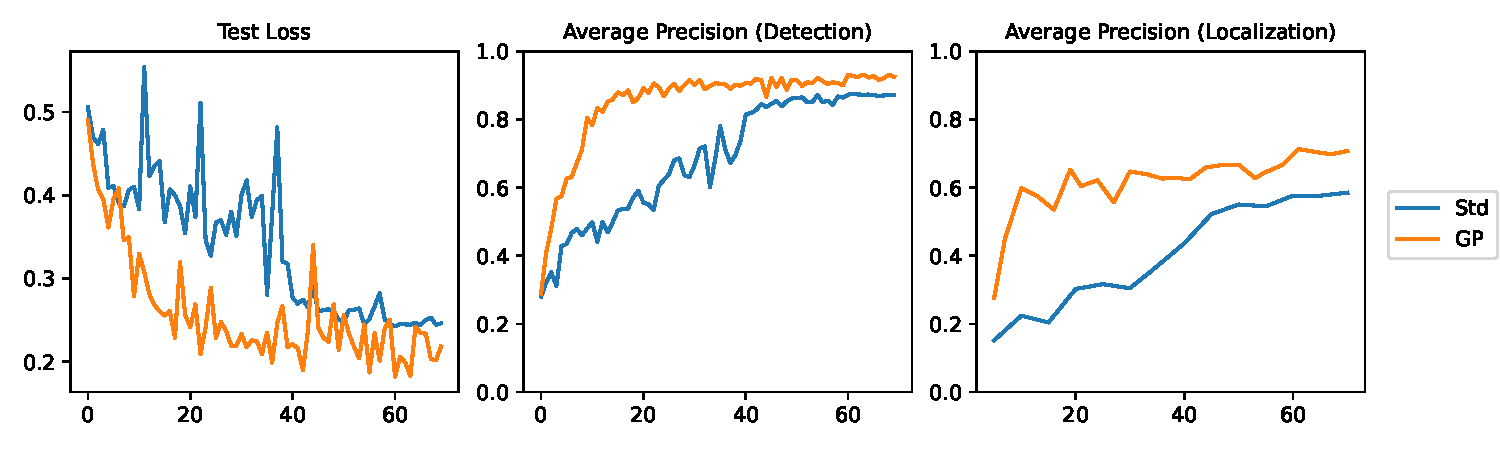
\includegraphics[width=15cm]{4_experiments/images/0_GP_exp/APs.pdf}
	\caption{(standard vs. optimized model) Progress of Test Loss and AP over epochs}
	\label{fig:gp_aps}
\end{figure}

\begin{figure}[h]
	\centering
	\makebox[\linewidth][c]{
		\begin{subfigure}[b]{1.2\textwidth}
			\centering
			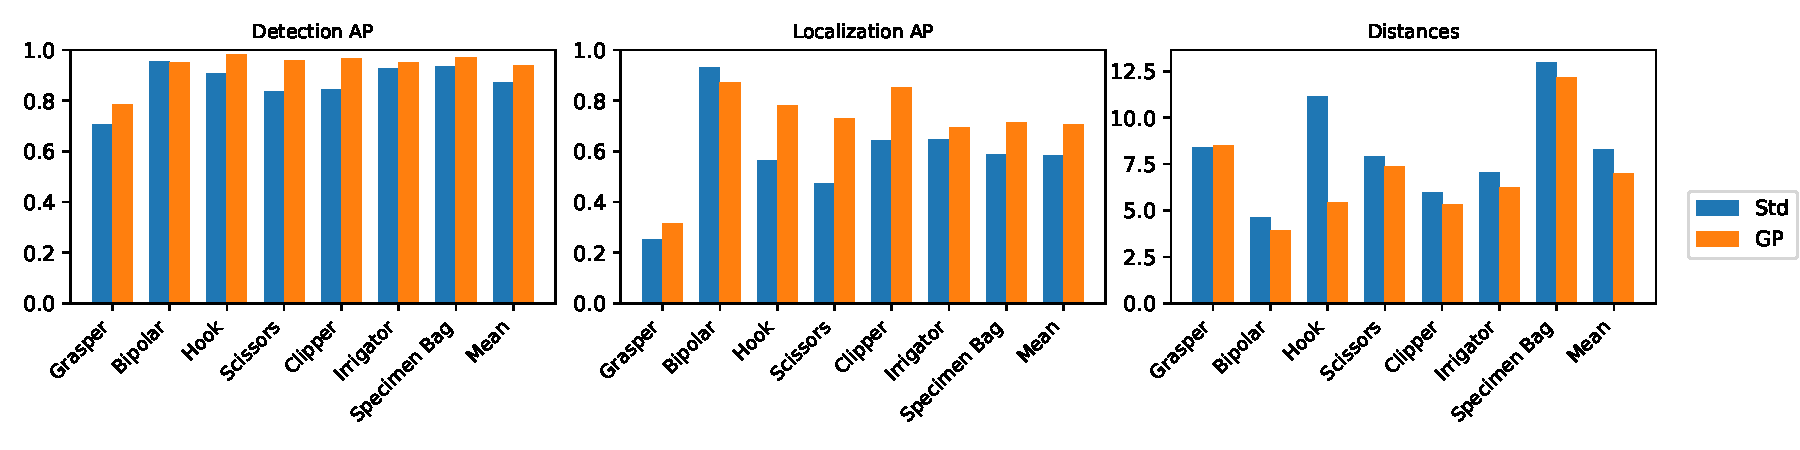
\includegraphics[width=18cm]{4_experiments/images/0_GP_exp/distances.pdf}
		\end{subfigure}
	}
\caption{(standard vs. optimized model) left: Classwise Average Precision of detection, middle: Classwise Average Precision of localization, right: Average distance between bounding box center and predicted position in \% of the image diagonal}
\label{fig:gp_distances}
\end{figure}

What we can see in \ref{fig:gp_aps}, is that one hand the model with optimized parameters seems to train a lot faster and more stable. While the test loss of the standard model sinks slow and with large peaks in between, the optimized one sinks very fast and converges then. The AP of the detection already reaches its maximum at about 30 epochs, while the other one achieves that after about 50. This is a major improvement for us, as our computing resources or scarce and training one model takes several hours. Because of this improvement we feel comfortable to lower the number of epochs to 50 instead of 70, as not much progress is made anymore after this point.\\
On the other hand, the optimized model also achieves a noticeable higher AP by about 6 percentage points for the detection and almost 12 for the localization.
Figure \ref{fig:gp_distances} shows us these differences for each class. Its noticeable that in both models, the \emph{Grasper} has much lower scores than the other tools. We guess this is the case, because the \emph{Grasper} is often very small and easily confused with other artifacts, like seams or dried blood. The \emph{Bipolar} on the other hand achieves very high scores, probably because of its unique shape and color.\\ Besides an improvement in the AP, we can also see that the distances between the bounding boxes and peaks reduced noticeably, by about 1.5 percentage points of the image diagonal and even halved for the \emph{Hook}.\\

In \textbf{future experiments}, we will use this optimized parameter set for our standard model.

\FloatBarrier



\subsection{Strides}
In the next experiment, we will evaluate the influence of the stride values in the last two conv. layers of the backbone on the models performance. For that we compared our standard model of stride (1,1) to two different ones of stride (1,2) and (2,2). They result in the following heatmap size:

\begin{center}
	\begin{tabular}{ c | c }
		Strides & Heatmap size\\
		\hline  
		(1,1) & 44$\times$76\\
		(1,2) & 22$\times$38\\
		(2,2) & 11$\times$19\\
	\end{tabular}
\end{center}

Disclaimer: With stride (x,y) we don't mean stride x across axis 0 and y across axis 1, but rather, (x,x) in the second-to-last conv. layer of the backbone and (y,y) in the last.\\

\cite{Vardazaryan} and \cite{lstm} chose (1,1) to increase the accuracy peaks in the heatmaps. We can see in \ref{fig:strides_aps} and \ref{fig:strides_distances}, if this worked for us, too.

\begin{figure}[h]
	\centering
	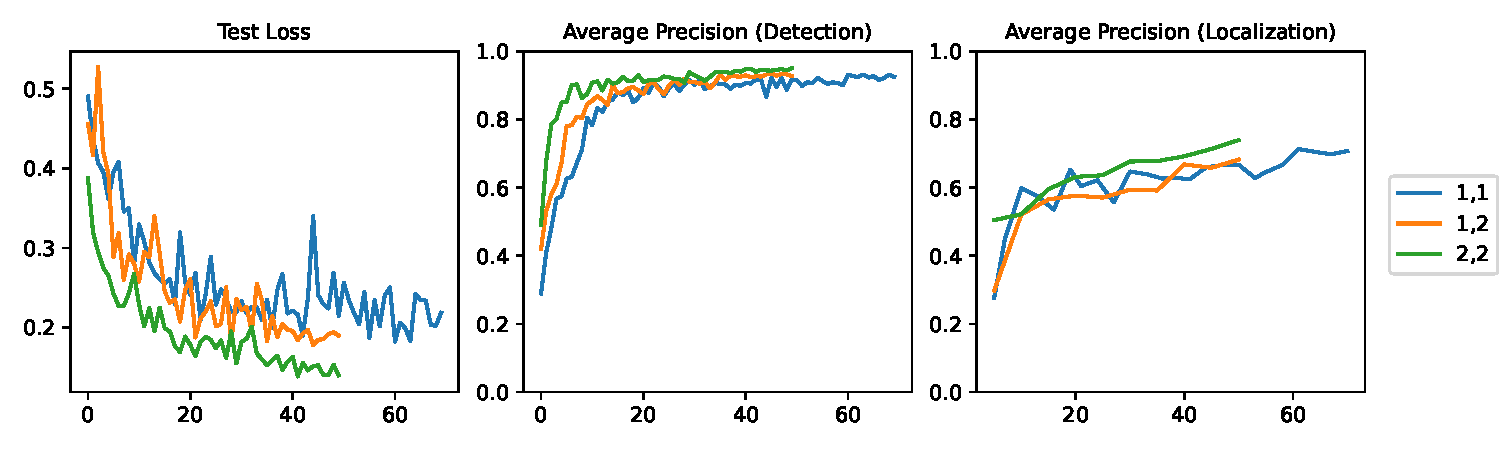
\includegraphics[width=15cm]{4_experiments/images/1_stride_exp/APs.pdf}
	\caption{(Stride (1,1) vs (1,2) vs (2,2)) Progress of Test Loss and AP over epochs}
	\label{fig:strides_aps}
\end{figure}

\begin{figure}[h]
	\centering
	\makebox[\linewidth][c]{
		\begin{subfigure}[b]{1.2\textwidth}
			\centering
			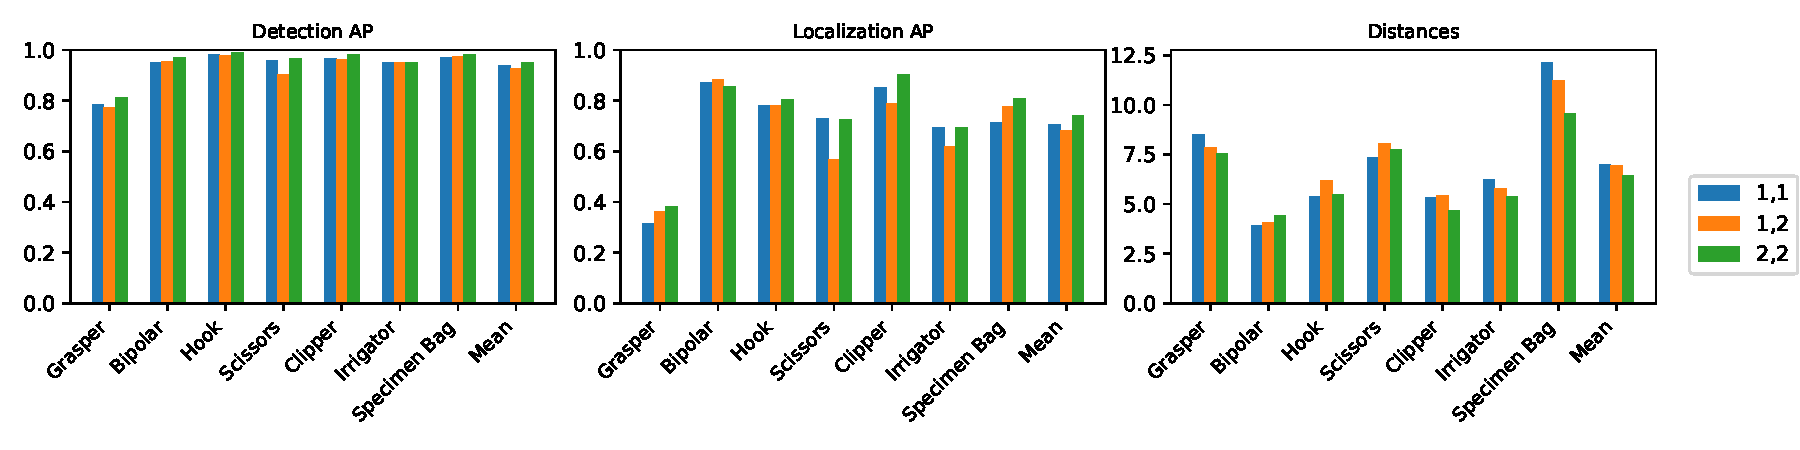
\includegraphics[width=18cm]{4_experiments/images/1_stride_exp/distances.pdf}
		\end{subfigure}
	}
	\caption{(Stride (1,1) vs (1,2) vs (2,2)) left: Classwise Average Precision of detection, middle: Classwise Average Precision of localization, right: Average distance between bounding box center and predicted position in \% of the image diagonal}
	\label{fig:strides_distances}
\end{figure}

As can be seen in \ref{fig:strides_aps} using strides (2,2) brings again a noticeable improvement over the current standard model of stride (1,1) and that in every regard. The test loss converges faster and more stable, while the maximum AP lies higher and is reached faster.\\
In \ref{fig:strides_distances} we see, that especially the \emph{Specimen Bag} benefits, as its distance sunk by almost 3 percentage points, which in return increases its localization AP. 

\FloatBarrier
\subsection{Backbones}

While \cite{Vardazaryan} and \cite{lstm} chose a ResNet18 as their backbones and \cite{classpeak} a ResNet50, we wanted to find out if another of the popular classification networks could bring further improvements. We will compare the already mentioned ResNet18 and ResNet50, against a AlexNet and VGGNet16. The results are seen in \ref{fig:bb_aps} and \ref{fig:bb_distances}.


\begin{figure}[h]
	\centering
	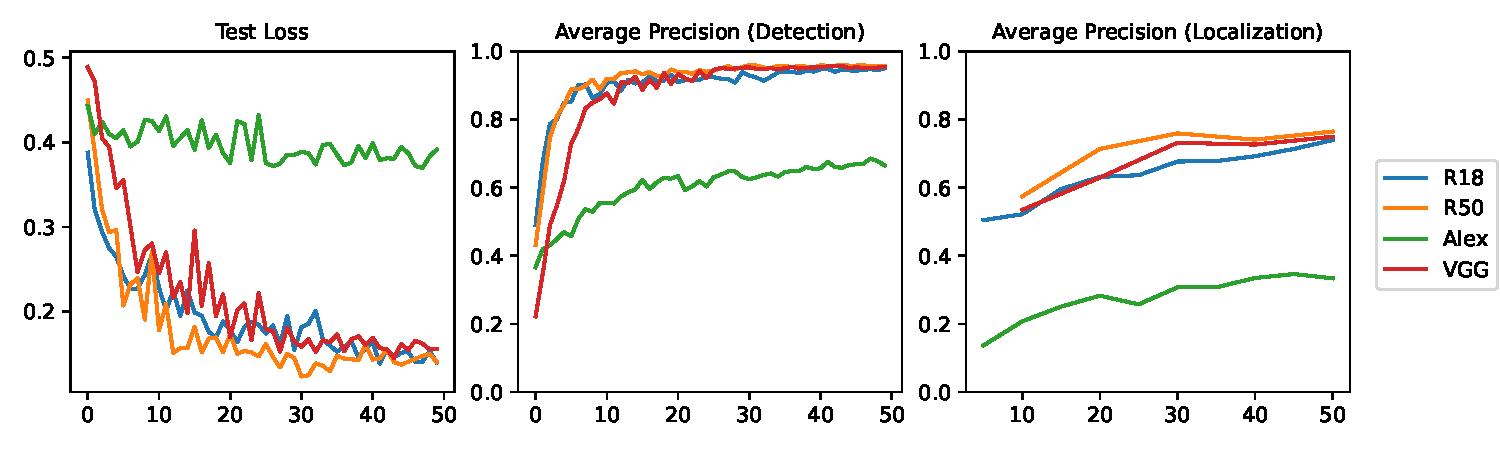
\includegraphics[width=15cm]{4_experiments/images/3_backbones/APs.pdf}
	\caption{(ResNet vs AlexNet vs VGGNet) Progress of Test Loss and AP over epochs}
	\label{fig:bb_aps}
\end{figure}

\begin{figure}[h]
	\centering
	\makebox[\linewidth][c]{
		\begin{subfigure}[b]{1.2\textwidth}
			\centering
			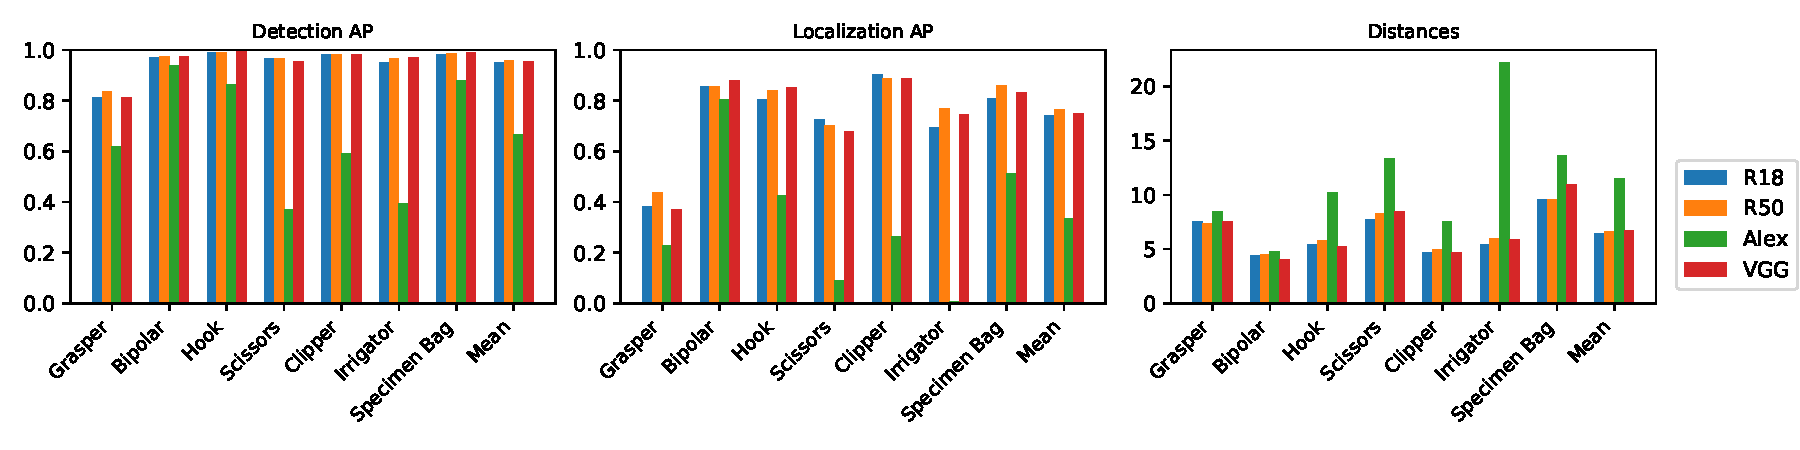
\includegraphics[width=18cm]{4_experiments/images/3_backbones/distances.pdf}
		\end{subfigure}
	}
	\caption{(ResNet vs AlexNet vs VGGNet) left: Classwise Average Precision of detection, middle: Classwise Average Precision of localization, right: Average distance between bounding box center and predicted position in \% of the image diagonal}
	\label{fig:bb_distances}
\end{figure}

Probably the most obvious result is, that the AlexNet performs a lot worse than all other 3 backbones. The reason for this is probably, that it is much simpler and and smaller than even the ResNet18, and is not able to learn as complex as the others. Interestingly, all other backbones perform roughly the same, even though ResNet50 and VGG16 are more complex networks, than the ResNet18. As they also require significantly longer training time and more memory, while giving barely any benefits, we will continue to use the ResNet18.

\FloatBarrier
\subsection{Spatial Pooling}
While \cite{Vardazaryan} examined the impact of WildCat \citep{Wildcat} instead of normal MaxPooling and showed that it performs better in most situations, we will instead compare WildCat to PeakResponse Pooling, which does not only take the highest peak in the heatmap into account, but also all the others with respect to their value.

\begin{figure}[h]
	\centering
	\makebox[\linewidth][c]{
		\begin{subfigure}[b]{1.2\textwidth}
			\centering
			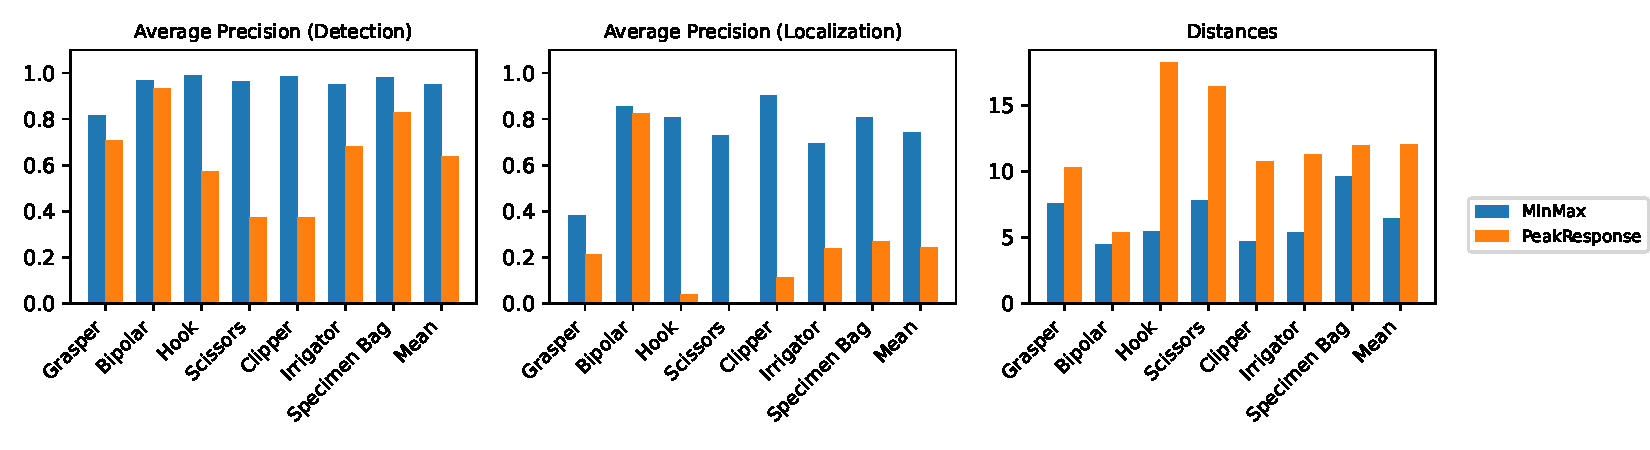
\includegraphics[width=18cm]{4_experiments/images/4_peak/AP.pdf}
		\end{subfigure}
	}
	\caption{(WilCat (MinMax) vs PeakResponse Pooling) left: Classwise Average Precision of detection, middle: Classwise Average Precision of localization, right: Average distance between bounding box center and predicted position in \% of the image diagonal}
	\label{fig:peak_distances}
\end{figure}

It stands out, that for every tool, except the \emph{Bipolar}, the PeakResponse Pooling performs significantly worse. This is surprising, as according to \cite{classpeak} it should actually perform better. Even though we reused the original implementation by the author, it is still possible, that this results occur due to a bug in our implementation.

\FloatBarrier
\subsection{Pre-Segmentation}

Another small change we hoped could improve our results, was to pre-segment a small number of images from the train dataset, by roughly deleting all parts of the image, that were of no interest for us (\ref{fig:seg_images}).

\begin{figure}[h]
	\centering
	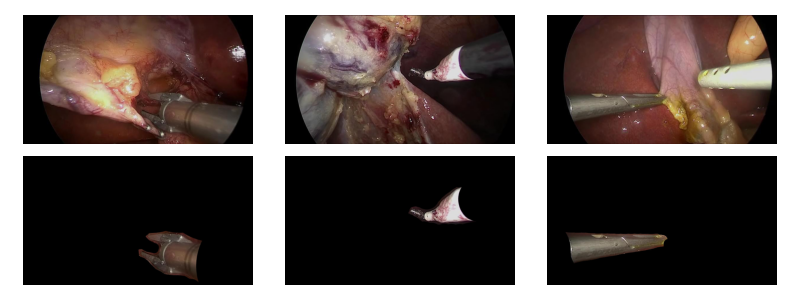
\includegraphics[width=15cm]{4_experiments/images/5_seg/images.png}
	\caption{A few examples of images pre-segmented images}
	\label{fig:seg_images}
\end{figure}

Our idea, was that we have three pre-segmented images for every class (working time: 20 minutes), that we train as one batch after every epoch of training. This should help our model to find the right tool, respectively the correct region of the tool. Our results can be seen in \ref{fig:seg_aps} and \ref{fig:seg_distances}.\\


\begin{figure}[h]
	\centering
	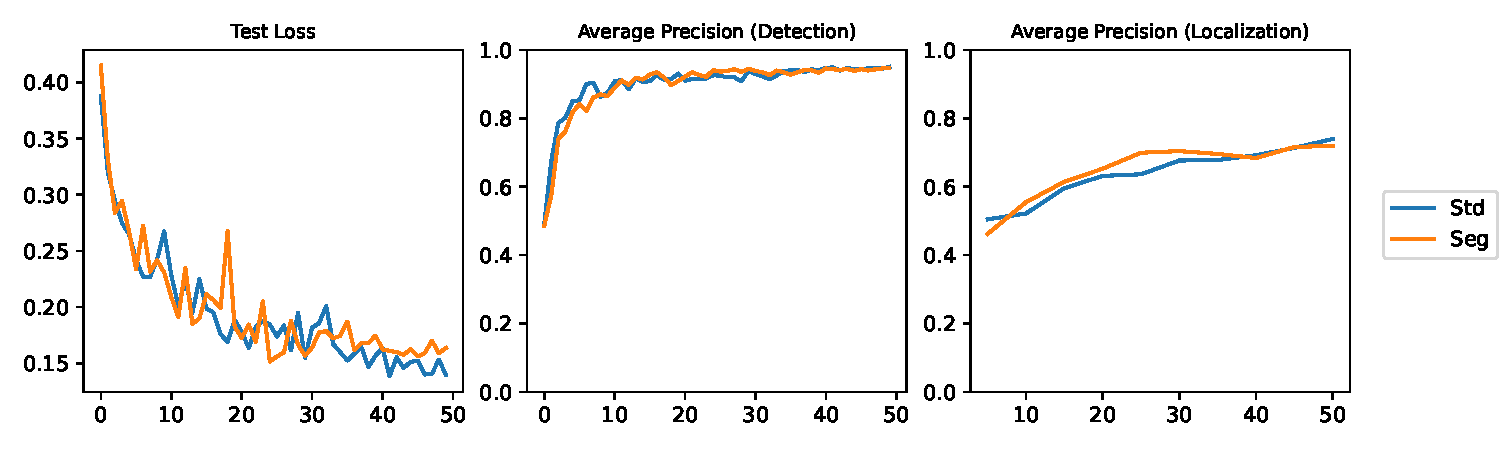
\includegraphics[width=15cm]{4_experiments/images/5_seg/APs.pdf}
	\caption{(Pre-Segmentation) Progress of Test Loss and AP over epochs}
	\label{fig:seg_aps}
\end{figure}

\begin{figure}[h]
	\centering
	\makebox[\linewidth][c]{
		\begin{subfigure}[b]{1.2\textwidth}
			\centering
			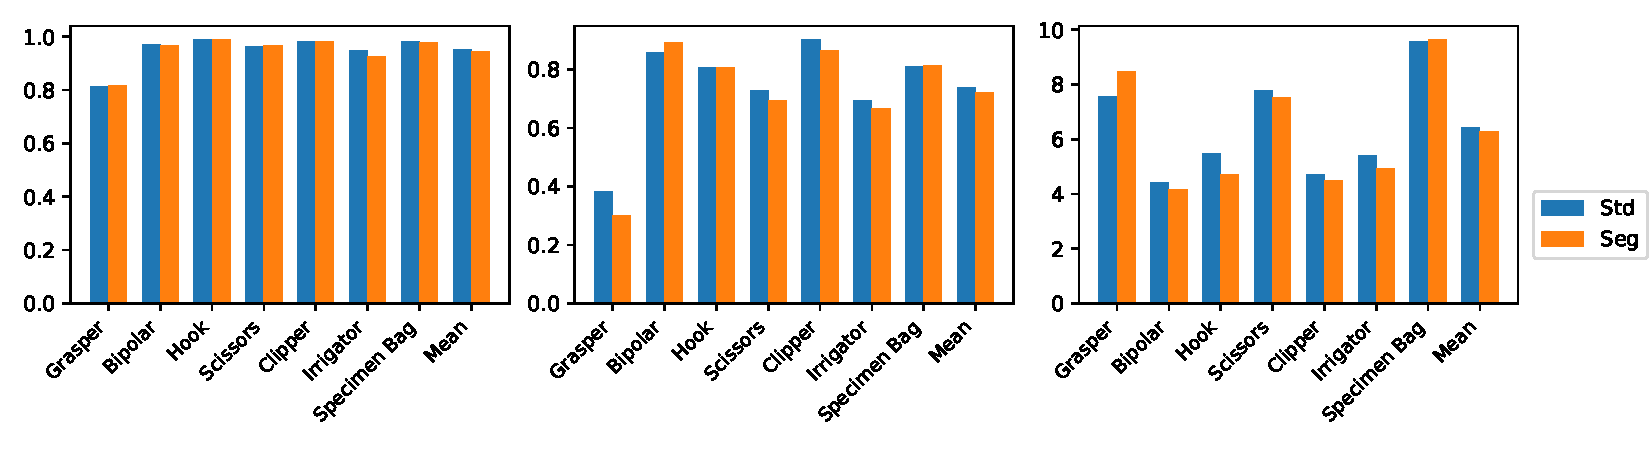
\includegraphics[width=18cm]{4_experiments/images/5_seg/distances.pdf}
		\end{subfigure}
	}
	\caption{(Pre-Segmentation) left: Classwise Average Precision of detection, middle: Classwise Average Precision of localization, right: Average distance between bounding box center and predicted position in \% of the image diagonal}
	\label{fig:seg_distances}
\end{figure}

Sadly, as can be seen theres barely any difference between the two results, so we can assume that pre-segmentation with such a small amount of images does have no impact.

\FloatBarrier
\subsection{ChannelSwitcher}

Our last experiment is based on the observation, that our tools are mostly gray, while everything around them has a dominant red channel. Our idea was, that if we randomly switch the color channels of the images during training, the model will be more likely to learn the features of not so much affected gray areas, instead of the strongly affected red areas.

\begin{figure}[h]
	\centering
	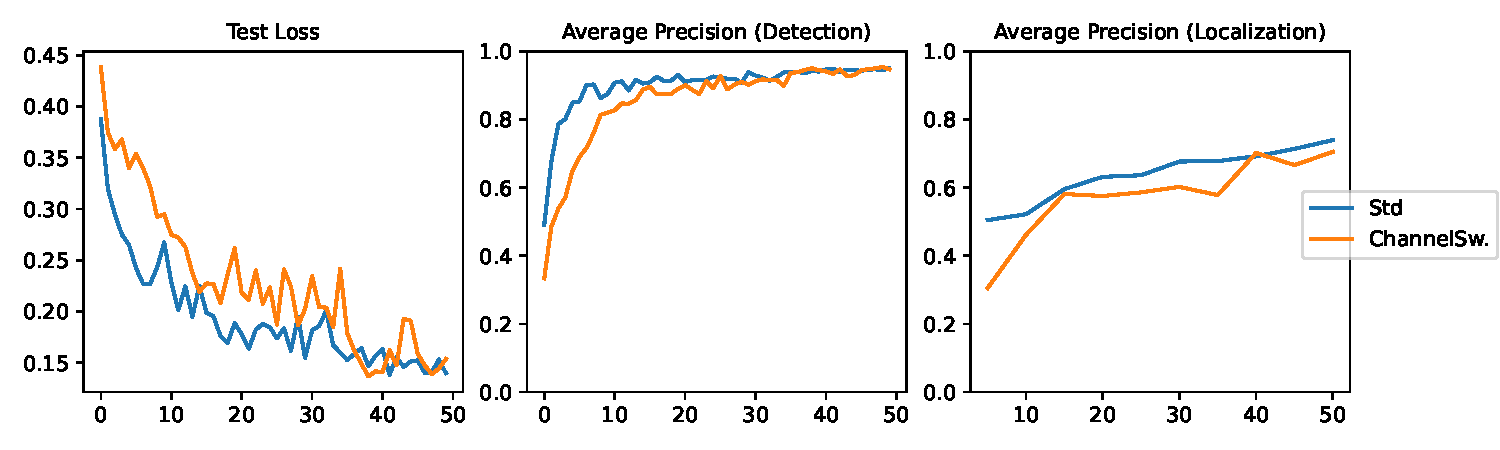
\includegraphics[width=15cm]{4_experiments/images/2_cs_exp/APs.pdf}
	\caption{(ChannelSwitcher) Progress of Test Loss and AP over epochs}
	\label{fig:cs_aps}
\end{figure}

\begin{figure}[h]
	\centering
	\makebox[\linewidth][c]{
		\begin{subfigure}[b]{1.2\textwidth}
			\centering
			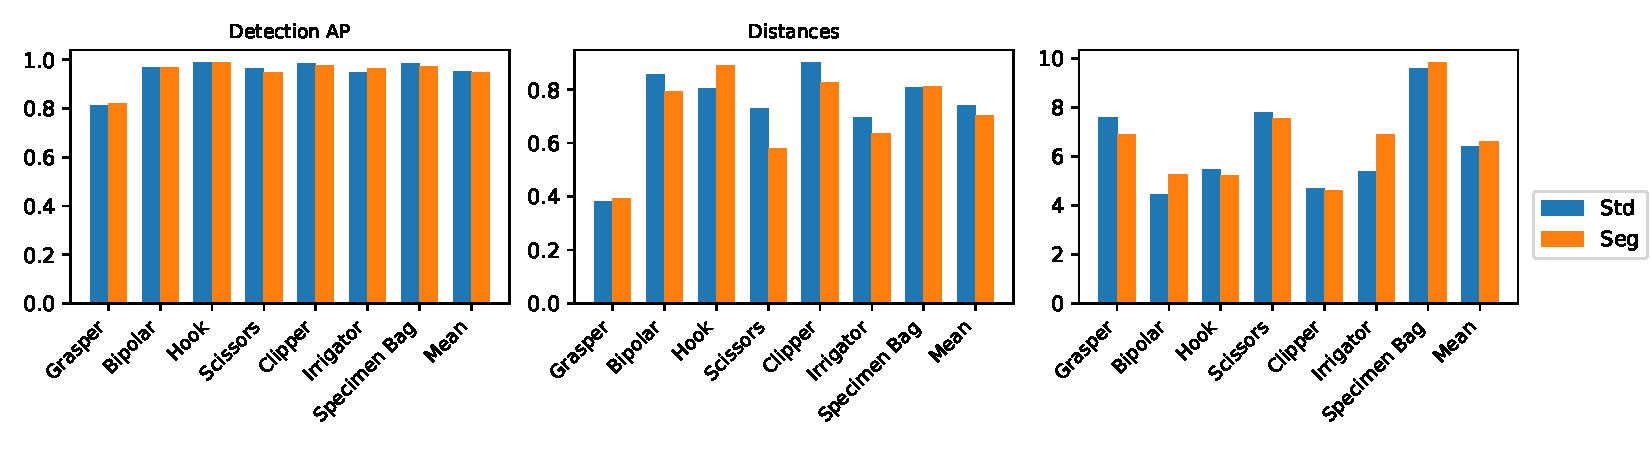
\includegraphics[width=18cm]{4_experiments/images/2_cs_exp/distances.pdf}
		\end{subfigure}
	}
	\caption{(ChannelSwitcher) left: Classwise Average Precision of detection, middle: Classwise Average Precision of localization, right: Average distance between bounding box center and predicted position in \% of the image diagonal}
	\label{fig:cd_distances}
\end{figure}


\FloatBarrier
\subsection{SurgToolLoc}


